\documentclass[11pt,a4paper]{article}

\usepackage[T1]{fontenc}
\usepackage[utf8]{inputenc}
\usepackage[a4paper,margin=2.2cm]{geometry}
\usepackage{graphicx}
\usepackage{booktabs}
\usepackage{array}
\usepackage{xcolor}
\usepackage{hyperref}
\usepackage{amsmath}
\usepackage{caption}
\usepackage{float}

\definecolor{azul}{HTML}{176B85}
\hypersetup{colorlinks=true,linkcolor=azul,urlcolor=azul,citecolor=azul}
\captionsetup{font=small,labelfont=bf}
\setlength{\parindent}{0pt}
\setlength{\parskip}{0.48em}
\renewcommand{\arraystretch}{1.12}
\renewcommand{\refname}{Fuentes y atribución}
\renewcommand{\tablename}{Tabla}
\renewcommand{\figurename}{Figura}

\begin{document}

\hypersetup{pageanchor=false}
\begin{titlepage}
\centering
\vspace*{3.2cm}
{\Large Memoria técnica\par}
\vspace{0.8cm}
{\Huge\bfseries Detección de superficies fotovoltaicas en cubiertas de Cantabria mediante ortofotografía aérea\par}
\vspace{1.2cm}
{\large De la transferencia de un modelo entrenado en Francia a indicadores municipales y producción estimada\par}
\vfill
\begin{tabular}{rl}
Autor: & \rule{8cm}{0.4pt}\\[0.7cm]
Fecha de entrega: & \rule{8cm}{0.4pt}
\end{tabular}
\vspace{2cm}
\end{titlepage}
\hypersetup{pageanchor=true}

\section{Resumen}

Se analizaron ortofotos PNOA 2023 de Cantabria para detectar superficie fotovoltaica sobre edificios catastrales. El primer intento consistió en aplicar directamente un modelo YOLO entrenado en Francia; su rendimiento cayó al pasar a Cantabria y motivó la creación de un conjunto local etiquetado. Tras comparar YOLO con dos versiones de U-Net, se eligió la U-Net con codificador ResNet34: en el test local obtuvo Dice 0,8560, IoU 0,7482 y un sesgo global de superficie del \(-7{,}54\,\%\).

La inferencia actual registra 3.188 edificios con detección entre 153.003 analizados y 202.786~m\textsuperscript{2} de superficie fotovoltaica planimétrica detectada. Una calibración experimental del sesgo eleva la estimación de superficie a 219.323~m\textsuperscript{2}. Bajo hipótesis comunes de potencia por superficie y rendimiento de PVGIS, el escenario central estima 43,86~MWp y 51,01~GWh anuales. Son estimaciones derivadas de imágenes, no registros de potencia instalada ni medidas de producción.

\section{Planteamiento y evolución}

El propósito inicial era localizar paneles en Cantabria reutilizando un detector YOLO entrenado con ejemplos franceses. La evaluación en Francia parecía suficiente para ensayar la transferencia, pero los resultados descendieron con fuerza al probarlo sobre imágenes cántabras.

% Fuente: cifras históricas facilitadas en el encargo de la memoria. No se localizó el archivo original de evaluación Francia--Cantabria en el repositorio.
\begin{table}[H]
\centering
\caption{Primera transferencia del modelo YOLO. Los valores proceden del registro facilitado para esta memoria; falta la salida original para verificarlos de forma independiente.}
\begin{tabular}{lrrrr}
\toprule
Prueba & Precisión & Recall & mAP50 & mAP50--95\\
\midrule
Validación en Francia & 0,717 & 0,857 & 0,787 & 0,468\\
Test en Cantabria & 0,339 & 0,321 & 0,257 & 0,149\\
\bottomrule
\end{tabular}
\end{table}

La caída indica un cambio de dominio. Podían influir la resolución, el aspecto de la ortofoto, los materiales de cubierta, la apariencia de los paneles, las condiciones de captura o la distribución de ejemplos. No hay un análisis que permita atribuirla a una causa concreta. El siguiente paso fue reunir ortofotos y etiquetas locales, entrenar un YOLO para Cantabria y desarrollar una U-Net de segmentación. La tabla anterior usa mAP de la primera fase; no es comparable directamente con Dice e IoU de la evaluación final por píxel.

\section{Datos}

La imagen de entrada procede de PNOA 2023 \cite{pnoa}. Los TIF usados tienen tres bandas RGB, sistema EPSG:25830 y píxeles de 0,15~m, comprobados en los archivos locales. Las huellas de edificios proceden de Catastro INSPIRE \cite{catastro}. El índice espacial contiene 100.591 teselas de hasta \(512\times512\) píxeles que intersectan algún edificio. En los bordes de las ortofotos puede haber ventanas menores.

Las imágenes seleccionadas se etiquetaron con polígonos en LabelMe. Para U-Net, cada etiqueta se convierte en una máscara binaria: un píxel marcado indica superficie fotovoltaica anotada y uno sin marcar indica fondo. La clase usada es \texttt{panel\_solar}. El mismo material etiquetado se exporta también al formato de segmentación de YOLO.

% Fuente: data/pool/manifest.csv y recuento directo de PNG en data/datasets/unet/masks/{train,val,test}.
\begin{table}[H]
\centering
\caption{Conjunto local usado en la comparación final. Los positivos se comprobaron en las máscaras actuales.}
\begin{tabular}{lrrr}
\toprule
Partición & Teselas & Positivas & Negativas\\
\midrule
Entrenamiento & 3.034 & 749 & 2.285\\
Validación & 744 & 26 & 718\\
Test & 988 & 31 & 957\\
\bottomrule
\end{tabular}
\end{table}

Cada identificador de tesela aparece una sola vez y la cuadrícula de 512 píxeles evita que dos teselas del índice compartan píxeles. El test se reservó como grupo separado; la validación actual se seleccionó entre muestras aleatorias. La separación no incluye un margen geográfico: el manifiesto muestra 37 teselas de test contiguas a alguna de entrenamiento o validación. Este límite se considera en la interpretación del test.

\section{Metodología}

Se entrenó una U-Net \cite{unet} con codificador ResNet34 \cite{resnet}. El codificador se creó con pesos ImageNet; la versión actual se ajustó a partir de los pesos de una U-Net anterior del proyecto. Las imágenes se leen en RGB, se dividen por 255 y se normalizan con media y desviación estándar ImageNet. La entrada es de \(512\times512\) píxeles y la máscara predicha se binariza con umbral 0,5. En entrenamiento se usan volteos y giros, pérdida BCE más Dice, optimizador AdamW y selección del mejor peso por Dice de validación.

El YOLO11s local \cite{yolo} se evaluó sobre el mismo test en términos de superficie segmentada por píxel. Para Cantabria se eligió la U-Net y se aplicó por ventanas: las predicciones se georreferencian, se acumulan sin contar dos veces las zonas compartidas y se intersectan con las huellas catastrales. Cada edificio se asigna a un municipio. El resultado conserva su geometría y superficies planimétricas; no cuenta instalaciones físicas individuales.

\section{Evaluación}

Las métricas finales se calcularon sumando \(TP\), \(FP\) y \(FN\) de todos los píxeles del test antes de formar los cocientes:
\[
\mathrm{Dice}=\frac{2TP}{2TP+FP+FN},\qquad
\mathrm{IoU}=\frac{TP}{TP+FP+FN}.
\]
\[
\mathrm{Precision}=\frac{TP}{TP+FP},\qquad
\mathrm{Recall}=\frac{TP}{TP+FN}.
\]
El sesgo de superficie implementado es
\[
b_A=\frac{A_{\mathrm{predicha}}-A_{\mathrm{anotada}}}{A_{\mathrm{anotada}}}
=\frac{(TP+FP)-(TP+FN)}{TP+FN}.
\]
Se expresa sobre el total del test, no como promedio de sesgos por imagen.

% Fuente: runs/evaluacion/unet_anterior/resumen.csv; runs/evaluacion/unet_actual/resumen.csv; runs/evaluacion/cantabria/yolo11s/revision/resumen.csv.
\begin{table}[H]
\centering
\caption{Comparación local por píxel sobre las mismas 988 teselas.}
\small
\begin{tabular}{lrrrrr}
\toprule
Modelo & Dice & IoU & Precisión & Recall & Sesgo de área\\
\midrule
U-Net anterior & 0,7944 & 0,6589 & 0,8869 & 0,7193 & \(-18{,}89\,\%\)\\
U-Net actual & \textbf{0,8560} & \textbf{0,7482} & \textbf{0,8909} & 0,8237 & \(-7{,}54\,\%\)\\
YOLO11s local & 0,7292 & 0,5739 & 0,6299 & \textbf{0,8658} & \(+37{,}45\,\%\)\\
\bottomrule
\end{tabular}
\end{table}

La U-Net actual mejora a la anterior en Dice, IoU y recall. YOLO encuentra una fracción algo mayor de los píxeles anotados, pero añade muchos más píxeles de fondo y sobreestima la superficie. Por eso la U-Net actual ofrece una base más equilibrada para indicadores de área. Su sesgo de \(-7{,}54\,\%\) significa que, en conjunto, predijo menos superficie de la anotada; no garantiza el mismo error en cada cubierta.

% Fuente: runs/evaluacion/unet_actual/resultados.csv; clasificación heurística en src/paneles_solares/modelos/evaluar_unet.py.
La revisión automática de imágenes clasificó 970 como aceptables, 10 como falsos positivos, 7 como falsos negativos y 1 como error mixto. Es una clasificación para inspección visual, distinta de las métricas por píxel.

% Fuente: runs/evaluacion/unet_actual/{falso_positivo,falso_negativo}/*.png; copias exactas en docs/figuras/.
\begin{figure}[H]
\centering
\begin{minipage}[t]{0.45\linewidth}
\centering
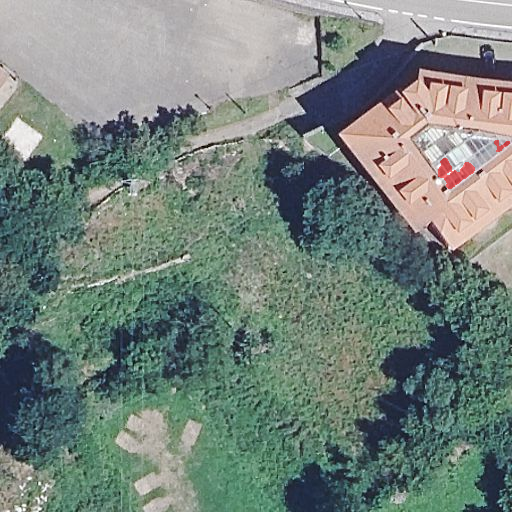
\includegraphics[width=\linewidth]{figuras/ejemplo_falso_positivo.png}\\
\small Predicción sobrante (rojo).
\end{minipage}\hfill
\begin{minipage}[t]{0.45\linewidth}
\centering
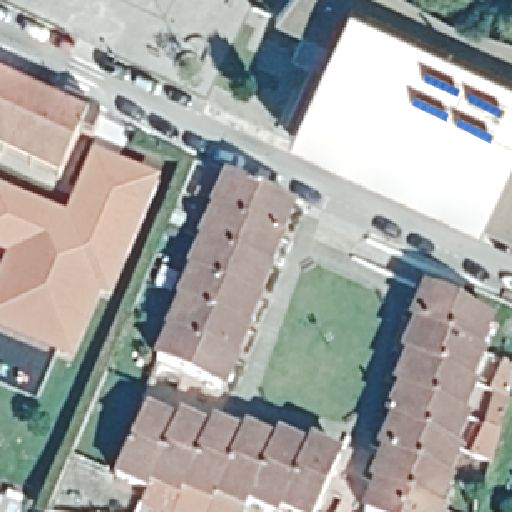
\includegraphics[width=\linewidth]{figuras/ejemplo_falso_negativo.png}\\
\small Superficie omitida (azul).
\end{minipage}
\caption{Dos errores guardados por la evaluación U-Net. Verde indica coincidencia cuando la hay.}
\end{figure}

\section{Indicadores territoriales}

Los GeoPackage conservan una fila por edificio y otra por municipio. Una cubierta con píxeles predichos tiene \emph{detección fotovoltaica}; una máscara puede fragmentar un grupo o unir varios, por lo que el número de edificios positivos no equivale al de instalaciones. El área se calcula en el plano proyectado a 0,15~m por píxel. La corrección \(A_{\mathrm{corr}}=A_{\mathrm{detectada}}/0{,}9246\) utiliza el sesgo redondeado del test como calibración experimental y mantiene separado el valor original.

% Fuente: runs/indicadores/unet_actual/municipios.csv y municipios.gpkg; totales de sus 102 filas.
\begin{figure}[H]
\begin{minipage}[c]{0.63\linewidth}
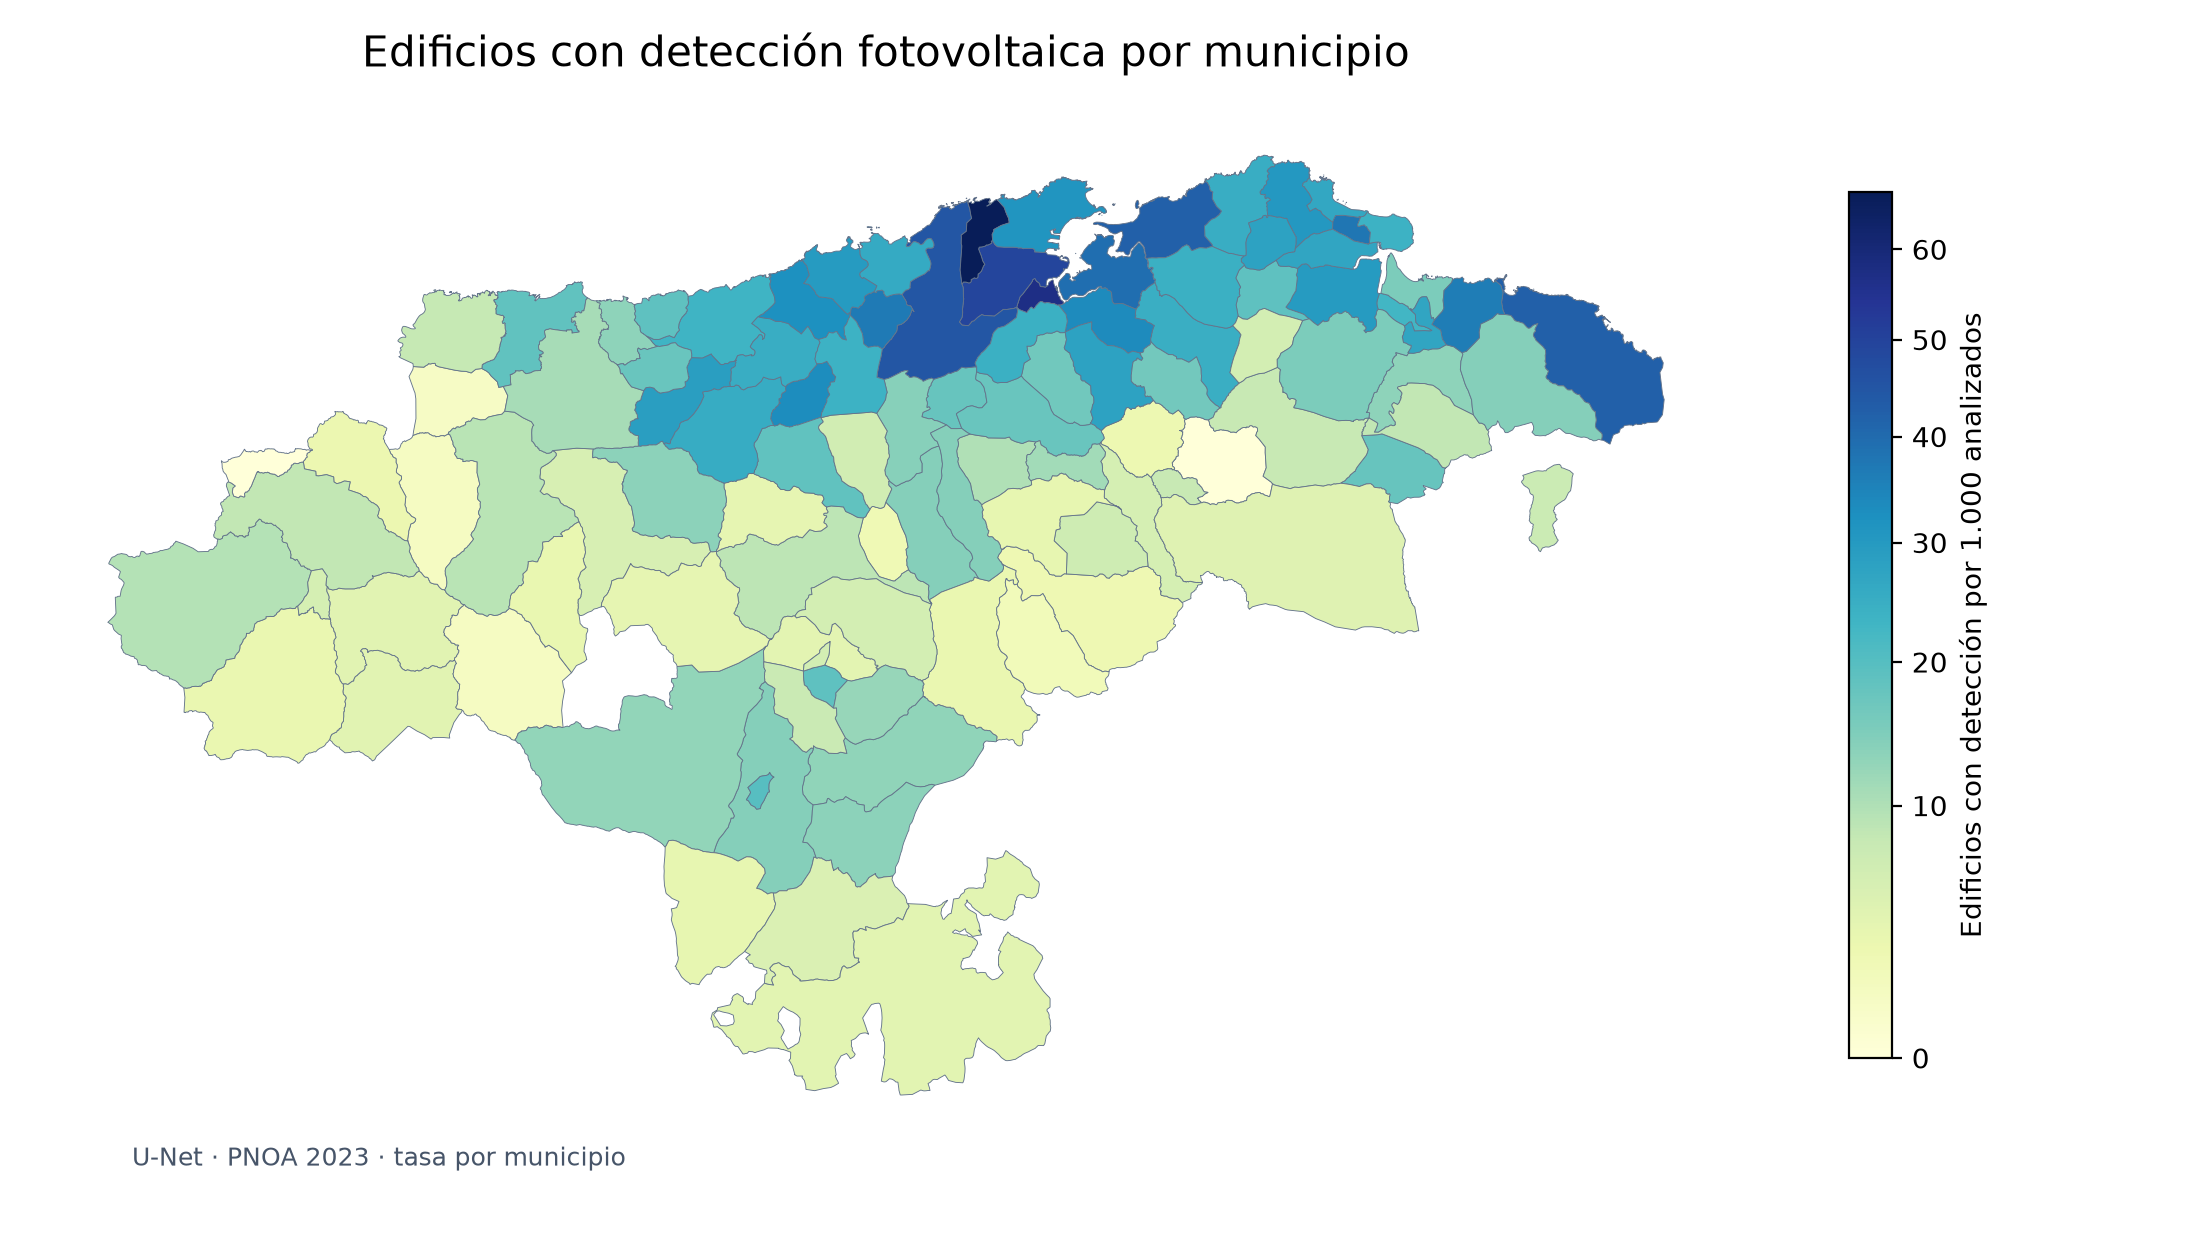
\includegraphics[width=\linewidth]{figuras/mapa_detecciones.png}
\end{minipage}\hfill
\begin{minipage}[c]{0.34\linewidth}
\small
\begin{tabular}{@{}lr@{}}
\toprule
Municipios & 102\\
Edificios analizados & 153.003\\
Con detección & 3.188\\
Proporción & 2,08\,\%\\
Por 1.000 edificios & 20,84\\
Área detectada & 202.786 m\textsuperscript{2}\\
Área corregida & 219.323 m\textsuperscript{2}\\
Cubierta ocupada & 0,51\,\%\\
\bottomrule
\end{tabular}
\end{minipage}
\caption{Distribución municipal de edificios con detección y resumen de Cantabria. El porcentaje de cubierta usa superficie detectada sin corregir. Límites municipales: IGN/CNIG.}
\end{figure}

% Fuente: runs/indicadores/unet_actual/municipios.csv; ordenado por superficie_fv_corregida_test_total_m2.
\begin{table}[H]
\centering
\caption{Municipios con mayor superficie fotovoltaica corregida.}
\begin{tabular}{lrrr}
\toprule
Municipio & Edificios positivos & Área corregida (m\textsuperscript{2}) & Por 1.000\\
\midrule
Santander & 335 & 28.720 & 31,2\\
Camargo & 223 & 18.335 & 49,3\\
El Astillero & 78 & 17.129 & 56,9\\
Polanco & 54 & 12.338 & 36,8\\
Medio Cudeyo & 67 & 10.938 & 33,5\\
\bottomrule
\end{tabular}
\end{table}

% Fuente: runs/indicadores/unet_actual/resumen_indicadores.png; copia exacta en docs/figuras/.
\begin{figure}[H]
\centering
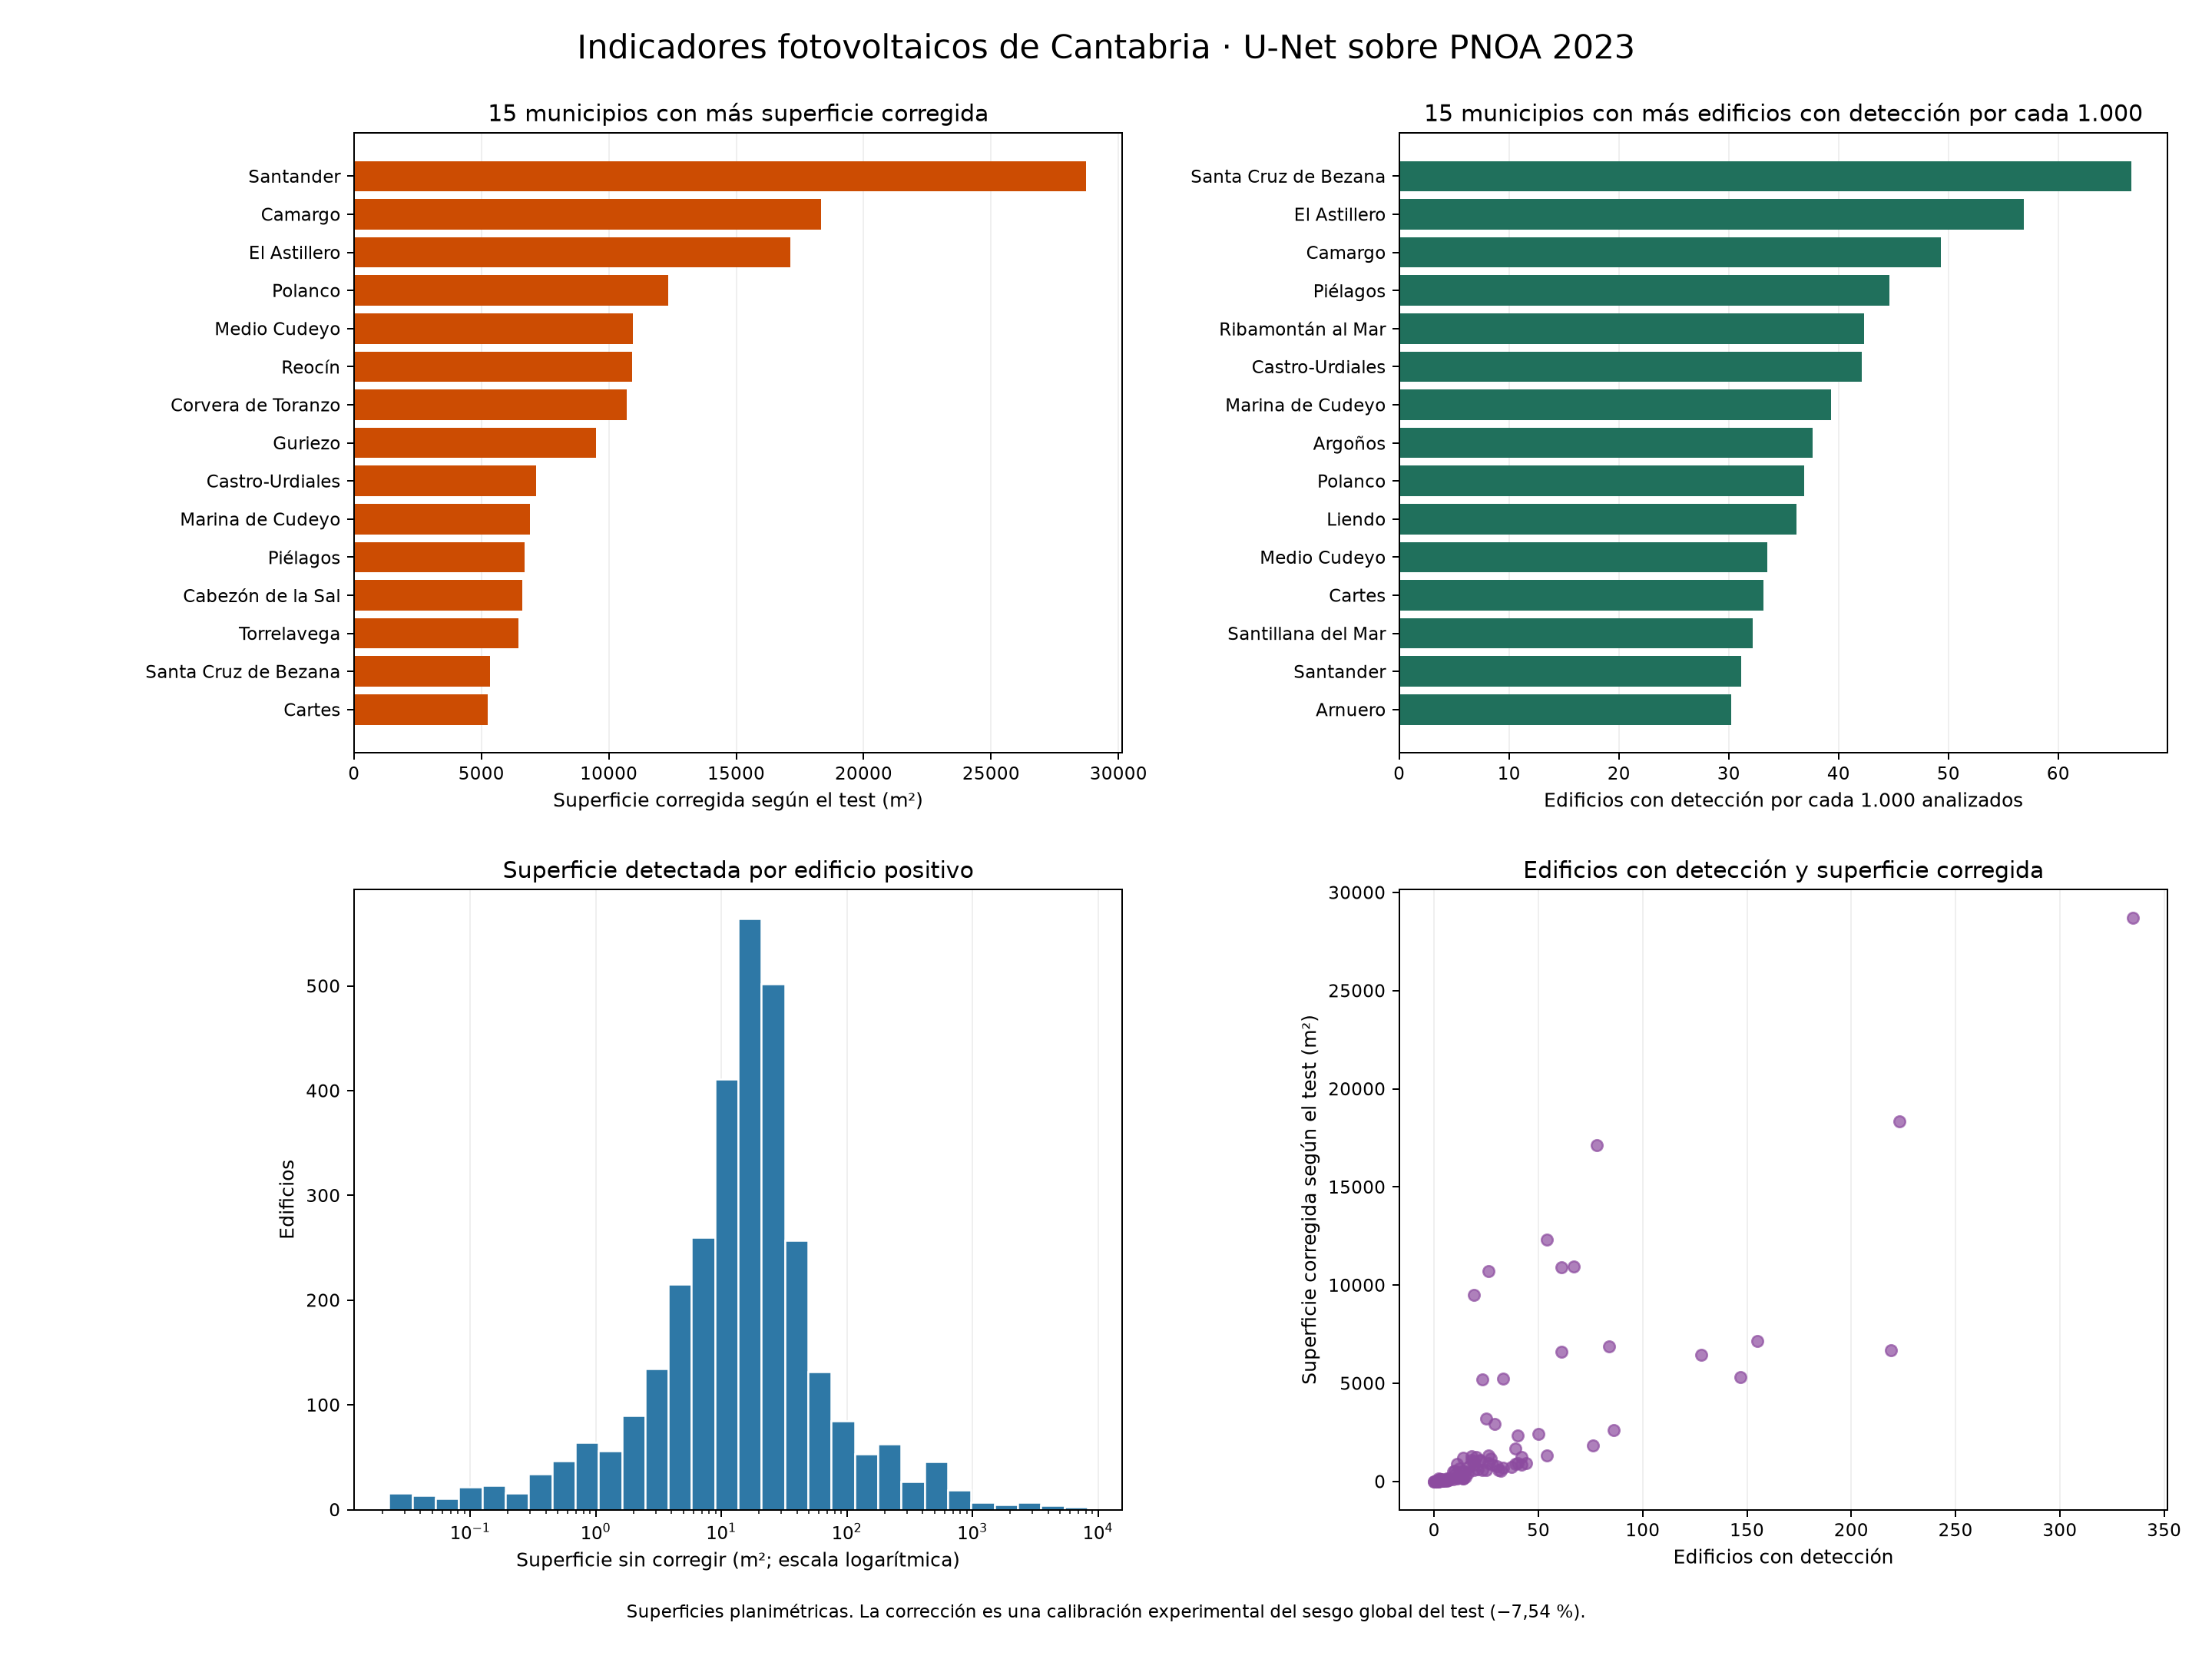
\includegraphics[width=\textwidth]{figuras/resumen_indicadores.png}
\caption{Superficies, tasas de detección y distribución entre edificios positivos. La superficie corregida no sustituye a la detectada.}
\end{figure}
\section{Potencia y producción estimadas}

La potencia pico no procede de registros eléctricos. Se aproxima a partir del área planimétrica asignada a cada municipio y una densidad efectiva:
\[
P_{\mathrm{kWp}}=A_{\mathrm{FV}}\,d_{\mathrm{kWp/m^2}},
\qquad
E_{\mathrm{kWh}}=P_{\mathrm{kWp}}\,Y_{\mathrm{PVGIS}}.
\]
\(Y_{\mathrm{PVGIS}}\) es el rendimiento de referencia en kWh/kWp. No se aplica una corrección geométrica adicional por inclinación.

% Fuente: runs/indicadores/unet_actual/produccion_config.json y produccion_municipal.csv.
\begin{table}[H]
\centering
\caption{Hipótesis de los tres escenarios. Las densidades son supuestos, no medidas.}
\begin{tabular}{lll}
\toprule
Escenario & Superficie usada & Densidad (kWp/m\textsuperscript{2})\\
\midrule
Conservador & Detectada sin corregir & 0,17\\
Central & Corregida con el test & 0,20\\
Superior & Corregida con el test & 0,23\\
\bottomrule
\end{tabular}
\end{table}

Para cada municipio con detecciones se consultó PVGIS 5.3 \cite{pvgis} con una posición media de edificios positivos ponderada por su área detectada. \texttt{PVcalc} dio doce rendimientos medios mensuales para 1~kWp. \texttt{seriescalc} aportó la forma horaria de 2019; cada mes de esa serie se normalizó hasta igualar el rendimiento mensual medio. El resultado contiene 8.760 horas UTC por municipio, pero es un \emph{perfil representativo}, no producción observada de 2019. Dos municipios sin detecciones tienen potencia y energía cero y no necesitan consulta.

Las condiciones comunes son 30\(^{\circ}\) de inclinación, orientación PVGIS 0\(^{\circ}\) (sur), pérdidas del 14\,\%, tecnología \texttt{crystSi} y base de radiación PVGIS-SARAH3. No se conocen la inclinación, orientación ni sombras reales de cada cubierta.

% Fuente: runs/indicadores/unet_actual/produccion_municipal.csv; sumas de 102 municipios. Comprobación con produccion_mensual.csv.
\begin{table}[H]
\centering
\caption{Totales estimados de Cantabria.}
\begin{tabular}{lrr}
\toprule
Escenario & Potencia pico (MWp) & Producción anual (GWh)\\
\midrule
Conservador & 34,47 & 40,09\\
Central & 43,86 & 51,01\\
Superior & 50,44 & 58,66\\
\bottomrule
\end{tabular}
\end{table}

% Fuente: runs/indicadores/unet_actual/municipios.gpkg y produccion_municipal.csv; mapa estático generado a partir de ambas salidas.
\begin{figure}[H]
\centering
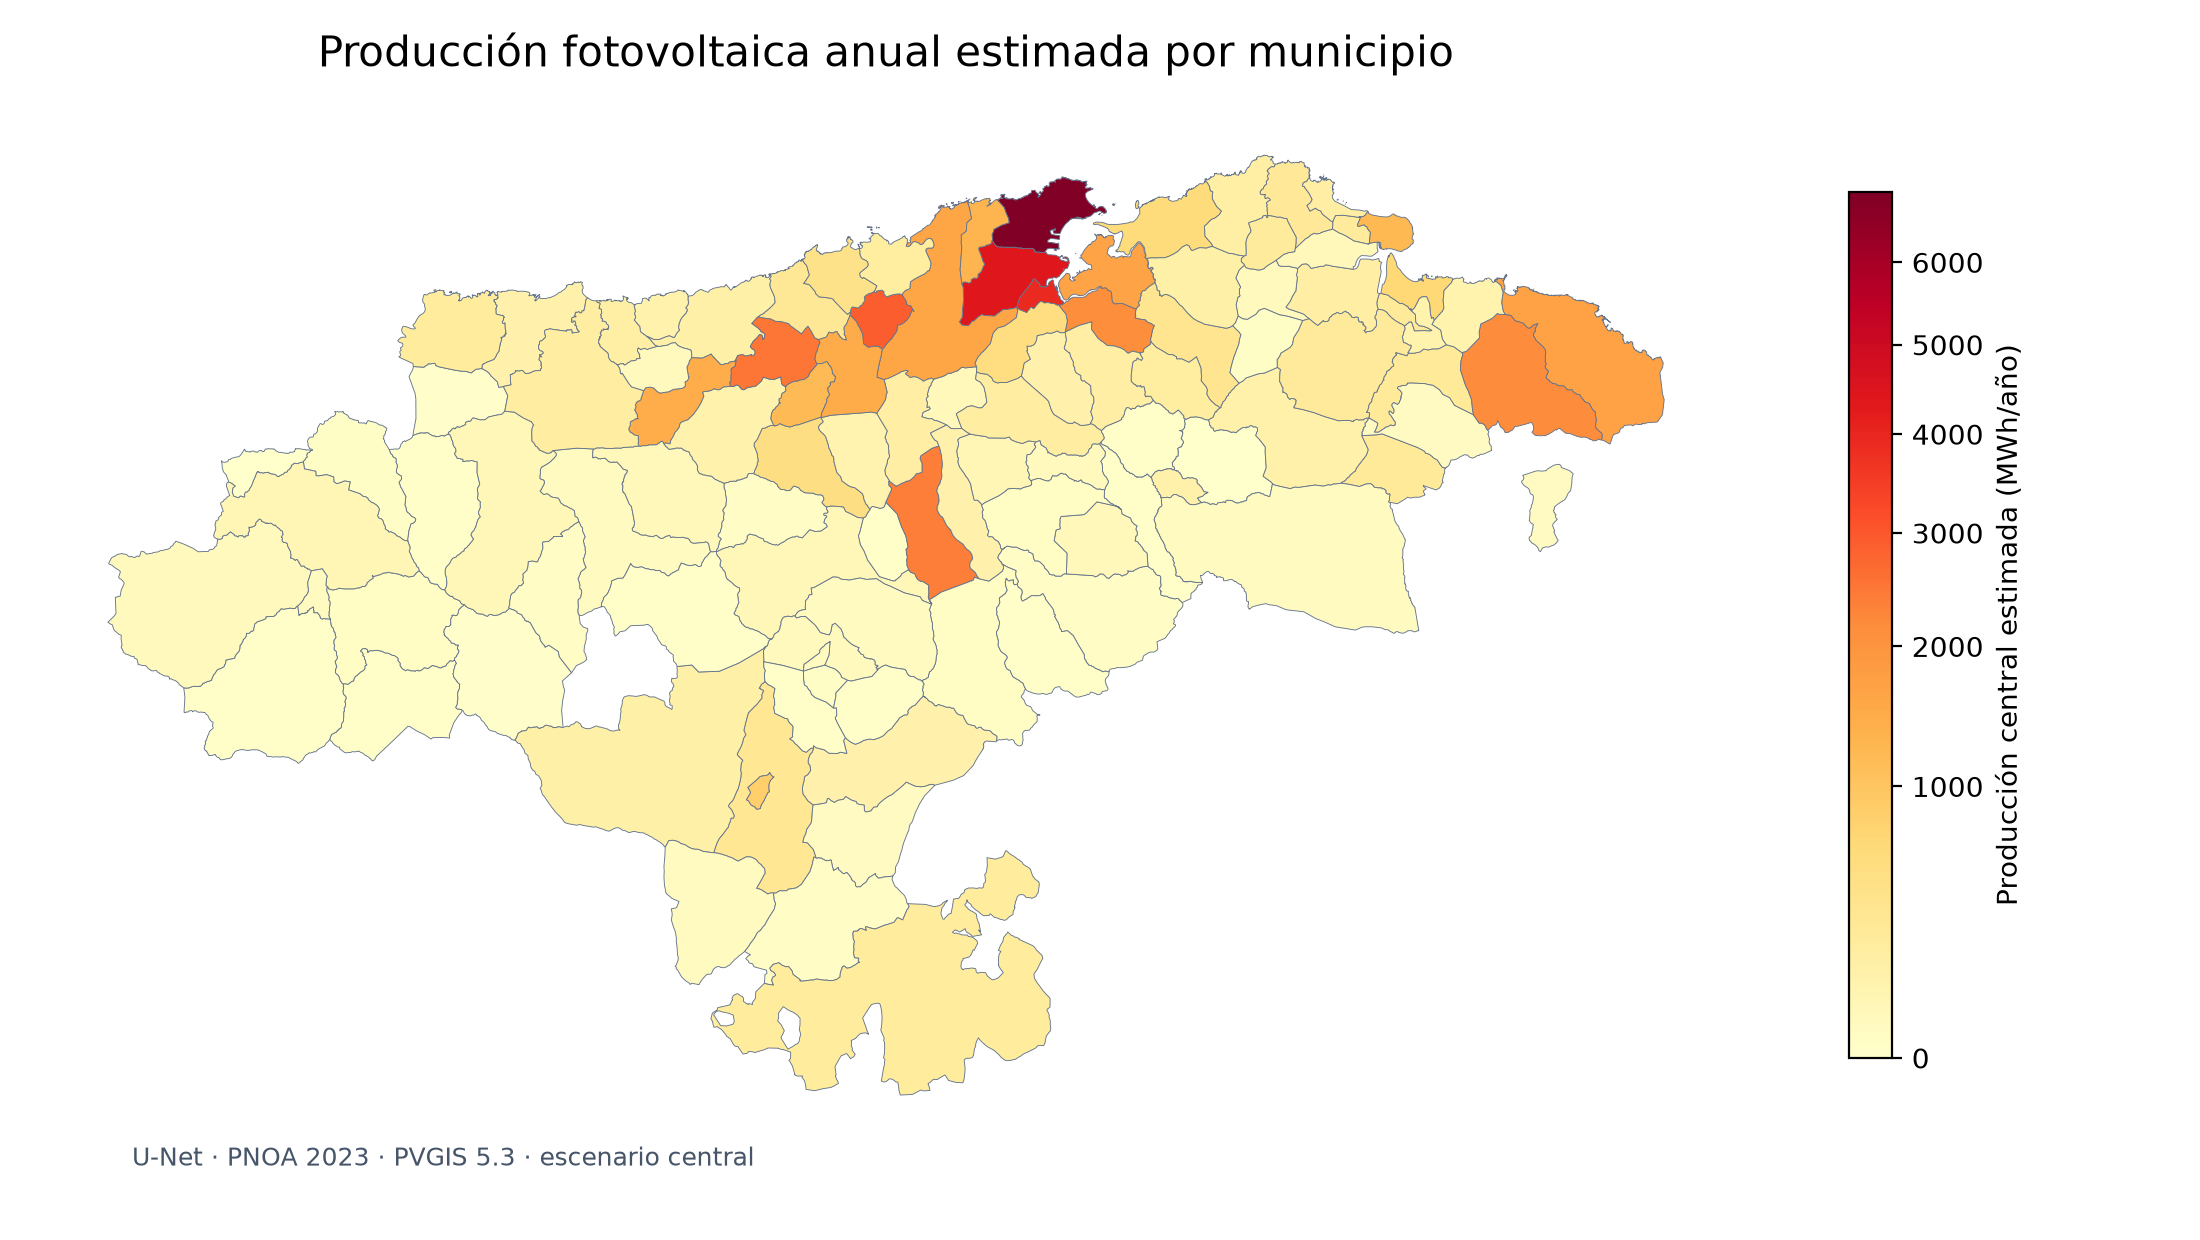
\includegraphics[width=0.96\textwidth]{figuras/mapa_produccion.png}
\caption{Producción anual central estimada por municipio. La escala colorea MWh/año, no potencia instalada. Límites municipales: IGN/CNIG.}
\end{figure}

% Fuente: runs/indicadores/unet_actual/produccion_municipal.csv; ordenado por produccion_anual_central_kwh.
\begin{table}[H]
\centering
\caption{Municipios con mayor producción anual estimada en el escenario central.}
\begin{tabular}{lrr}
\toprule
Municipio & Potencia central (MWp) & Producción central (GWh/año)\\
\midrule
Santander & 5,74 & 6,91\\
Camargo & 3,67 & 4,41\\
El Astillero & 3,43 & 3,94\\
Polanco & 2,47 & 2,92\\
Reocín & 2,18 & 2,51\\
\bottomrule
\end{tabular}
\end{table}

La producción mensual central total varía entre 2,54~GWh en enero y 5,47~GWh en julio, según \texttt{produccion\_mensual.csv}. La banda entre 40,09 y 58,66~GWh anuales expresa las tres hipótesis de superficie y densidad; no es un intervalo estadístico de confianza.

% Fuente: runs/indicadores/unet_actual/resumen_produccion.png, generado con produccion_municipal.csv, produccion_mensual.csv y produccion_horaria_representativa.csv; copia exacta.
\begin{figure}[H]
\centering
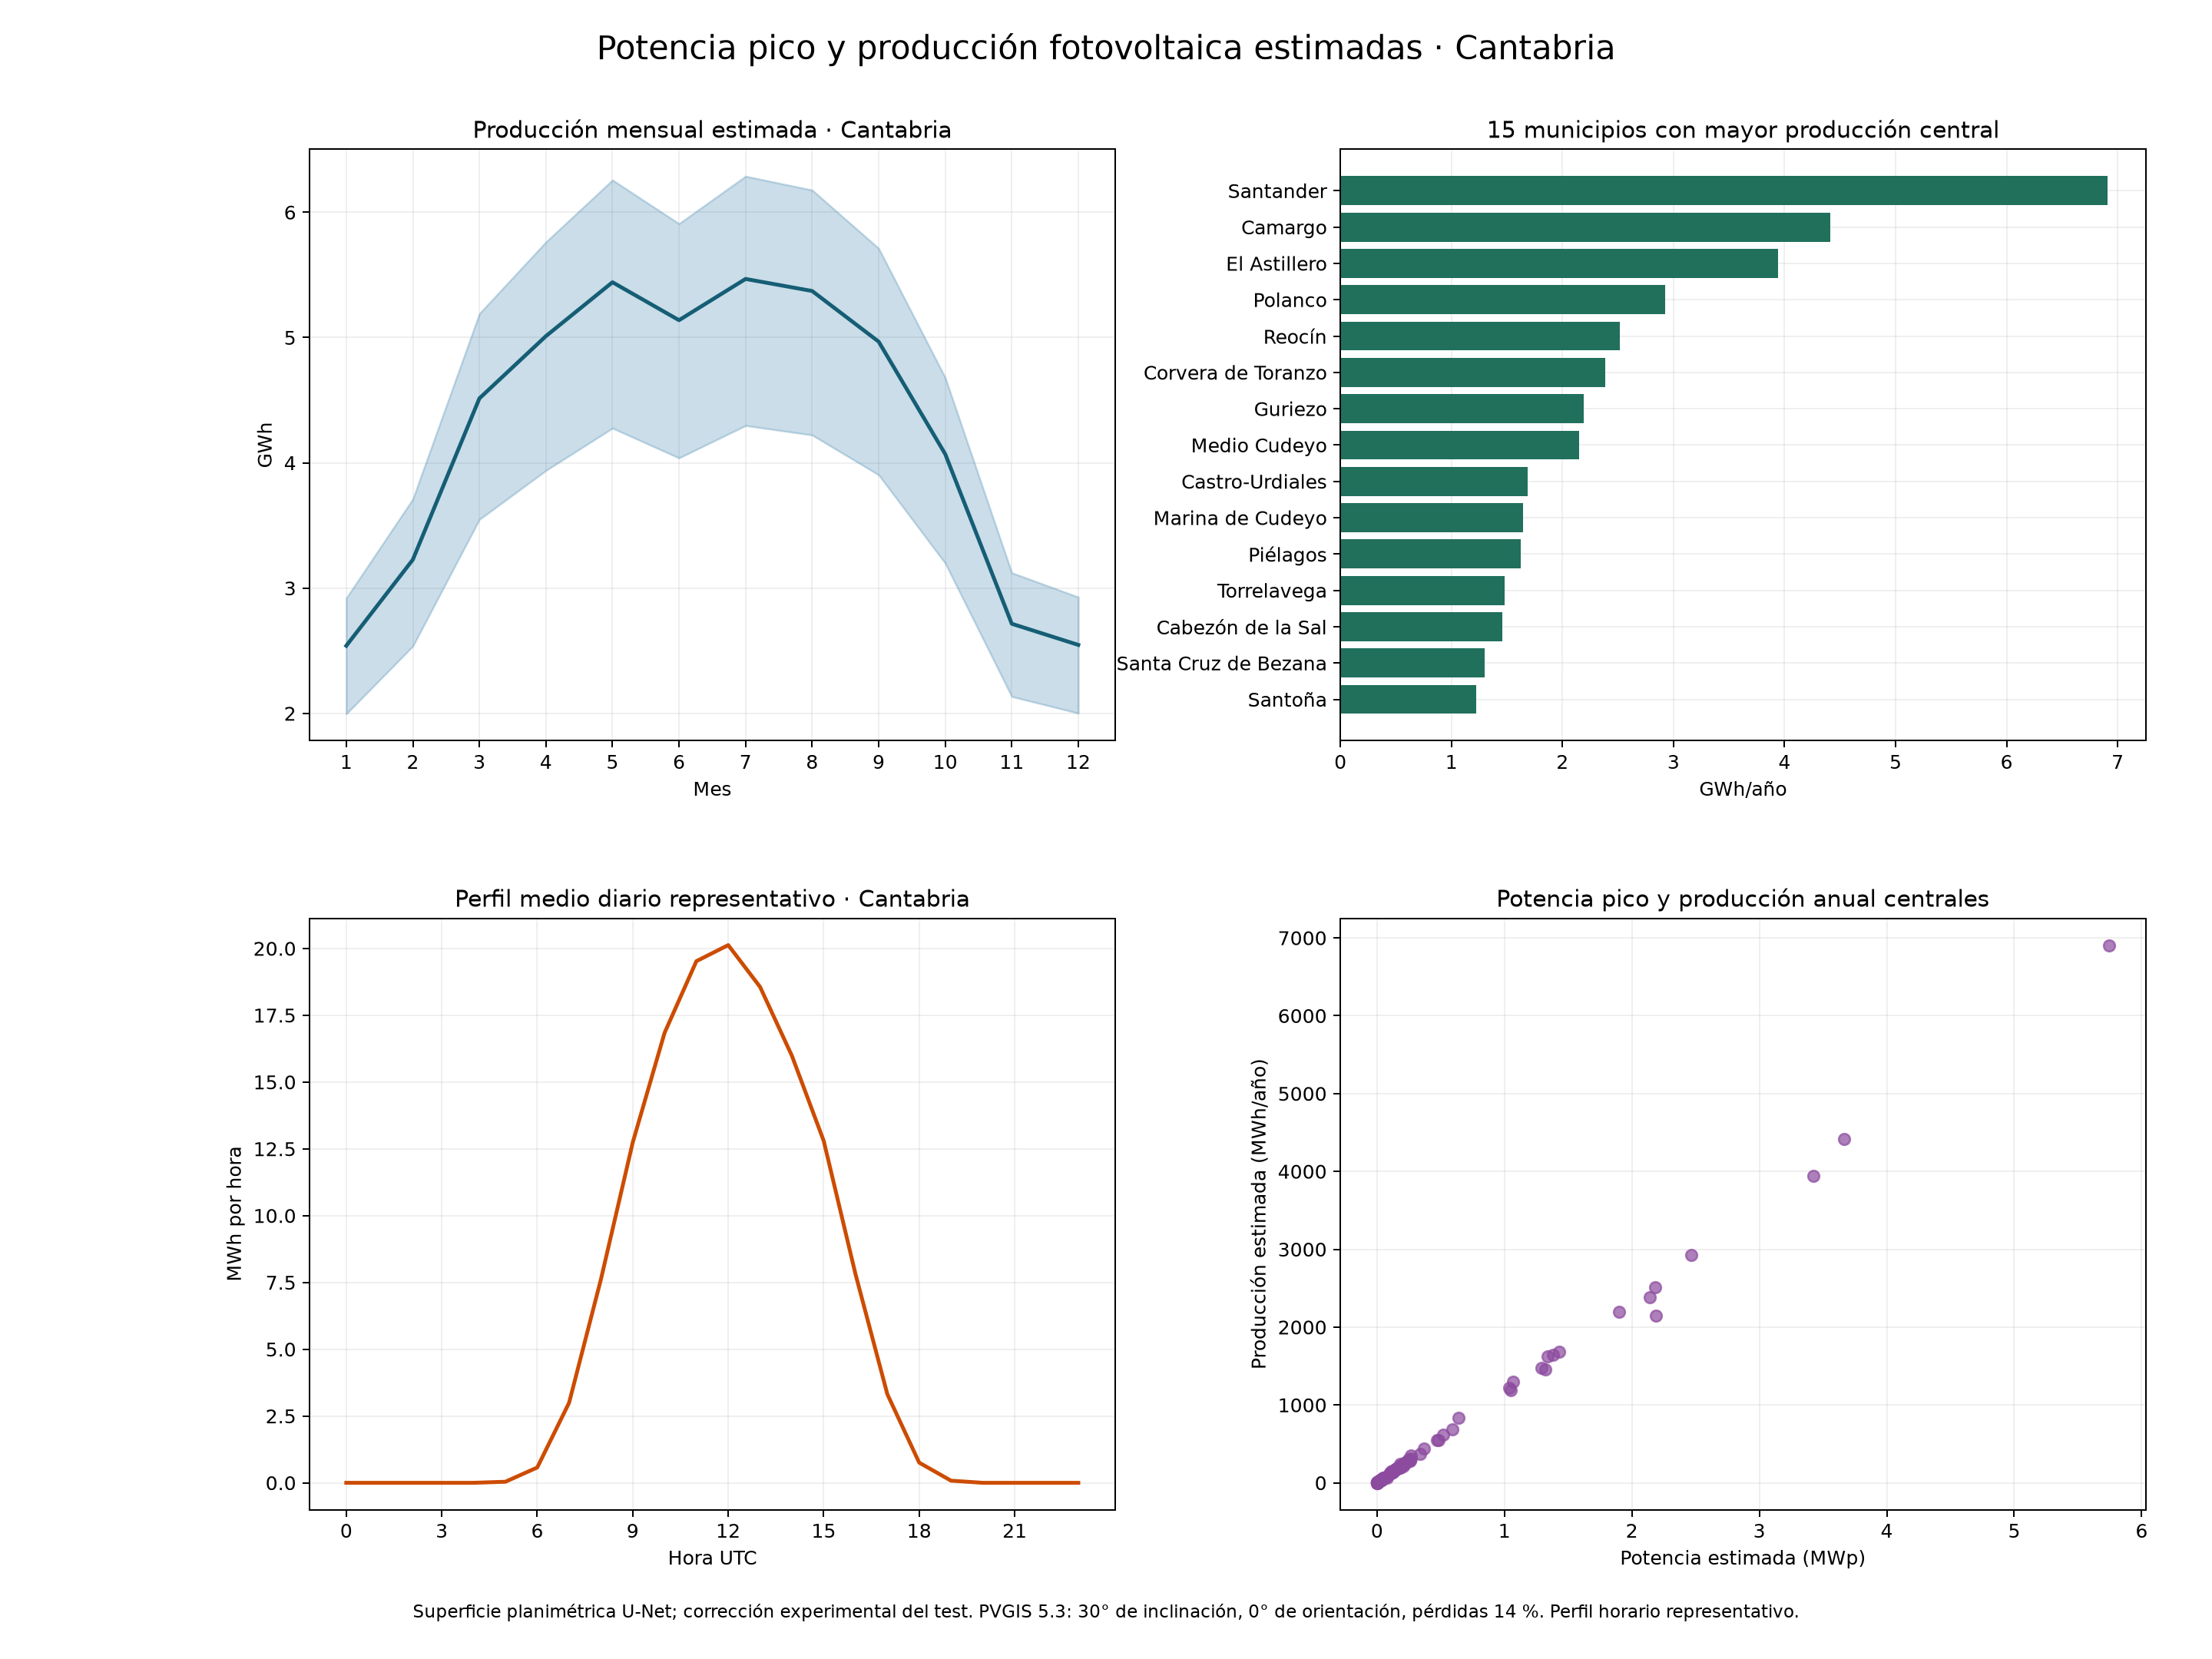
\includegraphics[width=\textwidth]{figuras/resumen_produccion.png}
\caption{Producción mensual y perfil diario de referencia, municipios principales y relación entre potencia y energía en el escenario central. La banda mensual une los escenarios conservador y superior.}
\end{figure}
\section{Limitaciones}

Solo 31 de las 988 teselas de test contienen paneles anotados (3,14\,\%). Aunque las 988 imágenes permiten una primera evaluación amplia de fondos y errores, ofrecen pocos positivos para estimar con precisión el rendimiento sobre paneles. Además, 37 teselas de test son contiguas a alguna tesela de entrenamiento o validación. La inferencia regional multiplica las oportunidades de falsos positivos al analizar muchas cubiertas. Conviene revisar visualmente los municipios extremos antes de interpretar diferencias pequeñas.

La corrección del \(-7{,}54\,\%\) refleja el sesgo global de un test concreto. No convierte cada edificio en una medida exacta y su incertidumbre no está cuantificada. Con 0,15~m por píxel, estructuras pequeñas o bordes complejos pueden ser difíciles de segmentar. El área estimada es planimétrica y no representa la superficie inclinada real de los módulos.

La potencia depende de densidades supuestas. PVGIS aporta rendimientos de referencia bajo geometría y pérdidas homogéneas; no incorpora la orientación e inclinación propia de cada cubierta, sus sombras ni datos reales de equipos. Las huellas catastrales y las ortofotos pueden corresponder a momentos distintos. Por todo ello, el inventario registra \emph{cubiertas con detección}, no instalaciones verificadas.

\section{Conclusiones y trabajo futuro}

La transferencia directa del modelo francés no funcionó bien en Cantabria. El conjunto local permitió entrenar y comparar alternativas sobre una referencia común; la U-Net actual redujo el error de superficie y alcanzó Dice 0,8560. El inventario resultante describe edificios y municipios, mientras que los 43,86~MWp y 51,01~GWh/año centrales son estimaciones condicionadas por supuestos explícitos.

Como validación final se plantea reunir unas 1.000 teselas nuevas, elegidas completamente al azar y con separación espacial respecto a entrenamiento y validación. Después se podrán calcular intervalos de confianza, revisar municipios extremos, incorporar inclinación y orientación derivadas de LiDAR y ajustar el modelo con la siguiente cobertura PNOA disponible. Una comparación con registros oficiales requeriría comprobar previamente que ambos conjuntos describen las mismas fechas y unidades.

\begingroup\small
\begin{thebibliography}{9}
\bibitem{pnoa} Instituto Geográfico Nacional y Centro Nacional de Información Geográfica. \emph{Plan Nacional de Ortofotografía Aérea, PNOA Imagen}. \href{https://pnoa.ign.es/}{pnoa.ign.es}. Ortofotos y límites derivados: © IGN/CNIG; origen reconocido conforme a su \href{https://centrodedescargas.cnig.es/CentroDescargas/politica-datos}{política de datos}, compatible con CC BY 4.0.
\bibitem{catastro} Dirección General del Catastro. \emph{Servicios INSPIRE de edificios y licencia de acceso y uso}. \href{https://www.catastro.hacienda.gob.es/webinspire/index.html}{catastro.hacienda.gob.es/webinspire}. Los indicadores son un producto transformado; no son cartografía catastral oficial.
\bibitem{pvgis} Joint Research Centre, Comisión Europea. \emph{PVGIS 5.3: API non-interactive service}. \href{https://joint-research-centre.ec.europa.eu/photovoltaic-geographical-information-system-pvgis/using-pvgis-5/api-non-interactive-service_en}{Documentación de la API}.
\bibitem{unet} O. Ronneberger, P. Fischer y T. Brox. \emph{U-Net: Convolutional Networks for Biomedical Image Segmentation}, 2015. \href{https://arxiv.org/abs/1505.04597}{arXiv:1505.04597}.
\bibitem{resnet} K. He, X. Zhang, S. Ren y J. Sun. \emph{Deep Residual Learning for Image Recognition}. CVPR, 2016. \href{https://openaccess.thecvf.com/content_cvpr_2016/html/He_Deep_Residual_Learning_CVPR_2016_paper.html}{Versión abierta}.
\bibitem{yolo} Ultralytics. \emph{YOLO11: documentación de modelos y segmentación}. \href{https://docs.ultralytics.com/models/yolo11/}{docs.ultralytics.com/models/yolo11}.
\end{thebibliography}
\endgroup

\end{document}
